%%%%%%%%%%%%%%%%%%%%%%% file template.tex %%%%%%%%%%%%%%%%%%%%%%%%%
%
% This is a general template file for the LaTeX package SVJour3
% for Springer journals.          Springer Heidelberg 2010/09/16
%
% Copy it to a new file with a new name and use it as the basis
% for your article. Delete % signs as needed.
%
% This template includes a few options for different layouts and
% content for various journals. Please consult a previous issue of
% your journal as needed.
%
%%%%%%%%%%%%%%%%%%%%%%%%%%%%%%%%%%%%%%%%%%%%%%%%%%%%%%%%%%%%%%%%%%%
%
% First comes an example EPS file -- just ignore it and
% proceed on the \documentclass line
% your LaTeX will extract the file if required
\begin{filecontents*}{example.eps}
%!PS-Adobe-3.0 EPSF-3.0
%%BoundingBox: 19 19 221 221
%%CreationDate: Mon Sep 29 1997
%%Creator: programmed by hand (JK)
%%EndComments
gsave
newpath
  20 20 moveto
  20 220 lineto
  220 220 lineto
  220 20 lineto
closepath
2 setlinewidth
gsave
  .4 setgray fill
grestore
stroke
grestore
\end{filecontents*}
%
\RequirePackage{fix-cm}
%
%\documentclass{svjour3}                     % onecolumn (standard format)
%\documentclass[smallcondensed]{svjour3}     % onecolumn (ditto)
%\documentclass[smallextended]{svjour3}       % onecolumn (second format)
\documentclass[twocolumn]{svjour3}          % twocolumn
%
\smartqed  % flush right qed marks, e.g. at end of proof
%
\usepackage{amsmath,graphicx}
\usepackage{import}
\usepackage[ruled]{algorithm2e}
%
% \usepackage{mathptmx}      % use Times fonts if available on your TeX system
%
% insert here the call for the packages your document requires
%\usepackage{latexsym}
% etc.
%
% please place your own definitions here and don't use \def but
% \newcommand{}{}
%
% Insert the name of "your journal" with
% \journalname{myjournal}
%
\begin{document}

\title{Low-complexity, Multi Sub-band Digital Predistortion:
		\thanks{This work was supported by the Finnish Funding Agency for Technology
		and Innovation (Tekes) under the project “Future Small-Cell Networks using
		Reconfigurable Antennas (FUNERA).” This work was also supported in part
		by the US National Science Foundation under grants ECCS-1408370, ECCS-
		1232274, and CNS-1265332 in the WiFiUS program. The work was also
		funded by the Academy of Finland under the projects 288670 “Massive MIMO:
		Advanced Antennas, Systems and Signal Processing at mm-Waves,” 284694
		“Fundamentals of Ultra Dense 5G Networks with Application to Machine Type
		Communication,” and 301820 “Competitive Funding to Strengthen University
		Research Proles,” and by the Linz Center of Mechatronics (LCM) in the
		framework of the Austrian COMET-K2 programme..}
}
\subtitle{Novel Algorithms and SDR Verification}
%\titlerunning{Short form of title}        % if too long for running head

\author{Chance Tarver         \and
        Mahmoud Abdelaziz \and
        Lauri Anttila \and
        Mikko Valkama \and
        Joseph~R.~Cavallaro
}

%\authorrunning{Short form of author list} % if too long for running head

\institute{Chance Tarver and Joseph R. Cavallaro \at
	Department of Electrical and Computer Engineering\\
	Rice University, Houston, TX, 77005, USA\\
	\email{\{cat12,cavallar\}@rice.edu}           %  \\
	%             \emph{Present address:} of F. Author  %  if needed
	\and
	Mahmoud Abdelaziz, Lauri Anttila and Mikko Valkama \at
	Department of Electronics and Communication Engineering\\
	Tampere University of Technology, Finland
}


\date{Received: date / Accepted: date}
% The correct dates will be entered by the editor

\maketitle

%Need to revise to include update.
%Current number of words: 138. 
%Recommended: 150 to 250 word
\begin{abstract}
The nonlinearities of power amplifiers combined with non-contiguous transmissions found in modern, frequency-agile, wireless standards create undesirable spurious emissions through the nearby spectrum of data carriers.
Digital predistortion (DPD) is an effective way of combating spurious emission violations without the need of a significant power reduction in the transmitter which can provide better power efficiency and network coverage. 
In this paper an iterative, multi sub-band version of the sub-band DPD, proposed earlier by the authors, is presented. 
The DPD learning is iterated over intermodulation distortion (IMD) sub-bands until a satisfactory performance is achieved for each of them. 
A sequential DPD learning procedure is also presented in order to reduce the hardware complexity when higher order nonlinearities are incorporated in the DPD learning. 
Improvements on the convergence speed of the adaptive DPD learning are also achieved via incorporating a variable learning rate and interpolation of previously trained DPD coefficients. 
A \textsc{Warp}Lab implementation of the proposed DPD is also shown with excellent suppression of the targeted spurious emissions. 
\keywords{Adaptive filters \and carrier aggregation \and digital predistortion \and nonlinear distortion \and power amplifier \and software-defined radio \and spectrally-agile radio \and spurious emission. }
% \PACS{PACS code1 \and PACS code2 \and more}
% \subclass{MSC code1 \and MSC code2 \and more}
\end{abstract}

\section{Introduction}
To meet increasing data-rate needs of mobile users, devices will need access to more of the radio spectrum. 
This is challenging considering the massive expected increase in the already large number of connected devices \cite{Cisco16}.
This leads to what is referred to as spectrum scarcity and fragmentation \cite{Staple04,Federated17}. 
In scenarios where there is little available bandwidth, it may be necessary to aggregate spectrum opportunistically, potentially across multiple bands non-contiguously. 
This sort of frequency-agile system has been adopted in protocols and standards such as in LTE-Advanced with carrier aggregation \cite{wannstrom_2013} and will likely also play a role in 5G communications \cite{Khan2014}.  

For cases where spectrum is aggregated in a non-continuous manner, challenges arise in the radio frontend design. 
In particular, the power amplifier (PA) becomes problematic. 
The PA is inherently a nonlinear device \cite{Ghannouchi09}, and whenever non-contiguous signals pass through this nonlinearity they intermodulate creating intermodulation distortion (IMD) components throughout the nearby spectrum as illustrated in Figure \ref{fig:PSD}. These spurious emissions or ``spurs" could interfere with other users or with a device's own receiver in a frequency-division duplexing scenario \cite{Park13}. 
This intermodulation distortion can be severe and violate emission requirements in standards such as the 3GPP LTE-Advanced or other FCC standards    \cite{Commag_abdelaziz,3GPP_CA_Emissions_1,3GPP_CA_Emissions_2,LaehteensuoMay2013}. 

\begin{figure}
	\centering
	%\vspace{0.5cm}
	\centerline{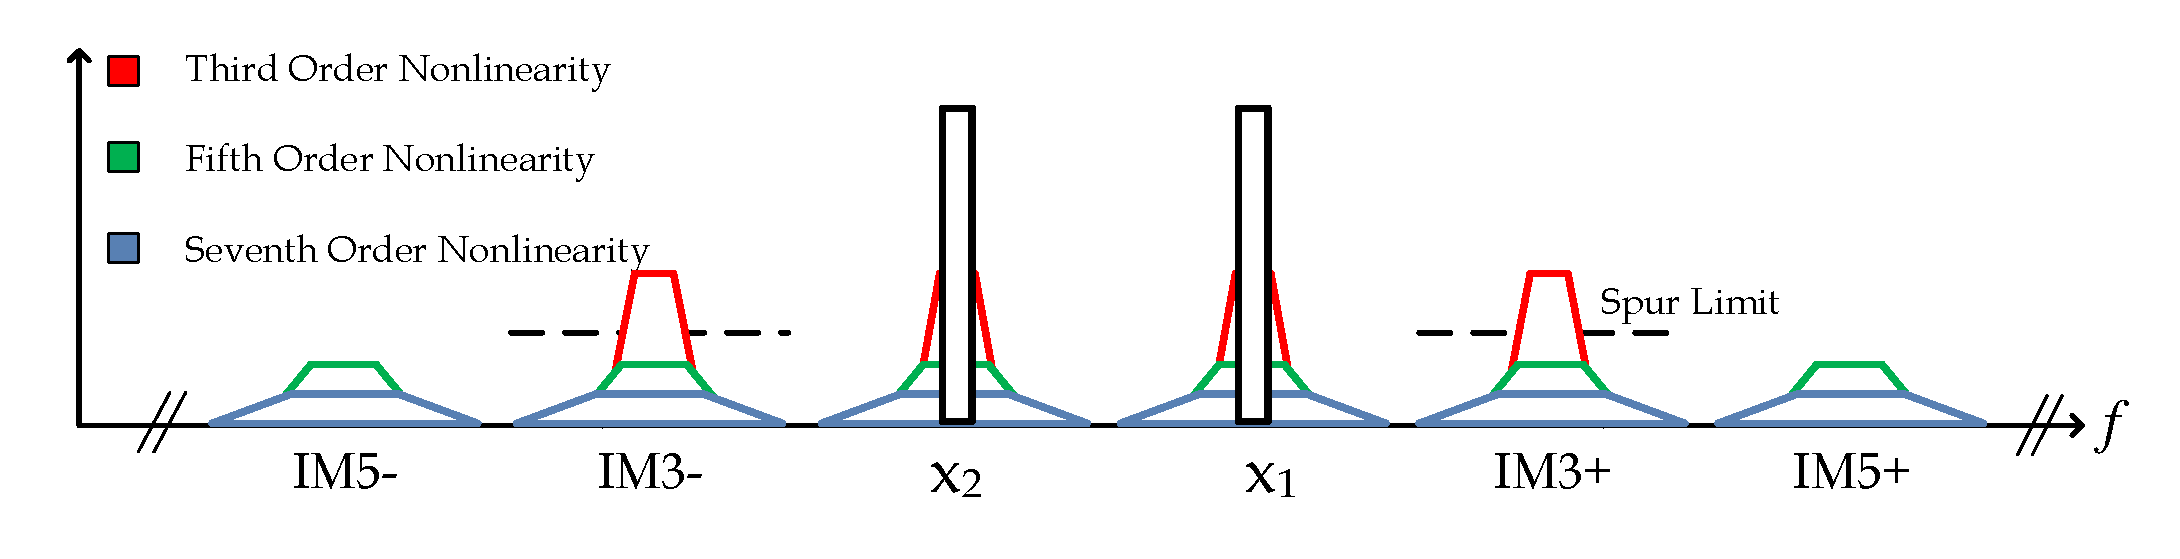
\includegraphics[width=\columnwidth]{PSD.pdf}}
	\caption[]{Power spectral density of a non-contiguous signal after being applied through a nonlinear PA.
		Nonlinearity orders up to the seventh are shown in the third-order and fifth-order intermodulation products (IM3 and IM5).}
	\label{fig:PSD}
\end{figure}

To avoid violating the strict emission requirements in such scenarios, devices may need to considerably back off their transmit power from the nominal maximum value (e.g., +23 dBm in 3GPP LTE uplink) so that the PA operates in a more linear region. 
However, reducing the transmit power in order to satisfy the emission mask will necessarily reduce the uplink coverage and the energy efficiency of the PA. 
 \cite{P.RoblinJan.2008,J.KimJan.2013,S.A.BassamAug.2012,ICASSP2014,Commag_abdelaziz,Katz16}. 

An alternative to power back-off is digital predistortion (DPD). 
DPD is a signal processing technique that requires sampling the output of the PA to learn its nonlinearities and then applying an inverse of them in the digital baseband signal to cancel the effect of the PA's nonlinearities. 
This can have the effect of dramatically reducing spurious emissions and other nonlinear effects \cite{Katz16}.

However, to cancel a nonlinearity, we have to also be able to observe it. For many carrier aggregation scenarios, the carriers may be spaced hundreds of MHz apart. 
This would lead to their intermodulation distortion products being spaced even farther apart so that the observation bandwidth necessary to mitigate the spurious emissions becomes infeasible for many analog-to-digital converters (ADCs) and radio-frequency (RF) downconverters \cite{S.A.BassamOct.2011}. 

This issue is quickly becoming more prevalent in that carrier aggregation is now almost commonplace. Since its 2011 debut in LTE Release 10, it has made its way from the standards down to commercial implementations. Many networks already provide support for up to three carriers on the downlink \cite{AT&T}, and many consumer devices also support it with system-on-chips such as the Snapdragon 835 supporting four downlink carriers and two uplink carriers \cite{Qual835}. 
However, most DPD solutions do not completely consider the carrier aggregation scenario. 
For example, in \cite{S.A.BassamOct.2011}, the effects of intermodulation are considered, but only the bandwidth around the main carrier is linearized. 

To combat this, the authors introduced a sub-band DPD method in \cite{ICASSP2014}. 
However, the third-order IMD (IM3) sub-bands were considered separately while not taking into consideration the mutual effect of each of the IM3 sub-band DPDs over the other. 
An \textsc{fpga} implementation of this solution has also been presented by the authors in \cite{Asilomar2015} demonstrating real-time processing of the adaptive DPD learning solution.

An extension of the DPD solution in \cite{ICASSP2014,Asilomar2015} was proposed in \cite{Tarver16}, where an iterative learning algorithm is used between the right and left IM3 sub-bands until they are both properly suppressed. 
A \textsc{Warp}Lab implementation of an iterative version of this higher order sub-band DPD was also presented  with additional ideas added to reduce the complexity and/or improve the learning speed of the proposed DPD. 
Moreover, in \cite{TMTT_SubbandDPD}, higher nonlinearity orders were introduced in addition to the third-order nonlinearity processing in \cite{ICASSP2014,Asilomar2015}. 

In this paper, we extend the work from \cite{Tarver16} to include processing for the fifth-order intermodulation products (IM5) and include new interpolation based speed-up methods. In summary, this paper includes:
\begin{itemize}
	\item An iterative version of the previously proposed sub-band DPD. This solution iterates between the different spurious components, such as the IM3+, IM3-, IM5+, and IM5- until a satisfactory performance is achieved for each of them. This improves the flexibility and potentially reduces complexity when compared to a full-band DPD system in that learning can be focused only on sub-bands that are in violation of emission limits. 
	\item The learning of the higher-order nonlinearities in each sub-band is done sequentially, one basis function at a time in ascending order. 
	This has the advantage of reducing the hardware complexity by essentially using one learning module for all the nonlinearity orders. 
	An additional flexibility advantage is that we can stop adding higher orders in the learning phase once a sufficient spurious emission suppression is achieved, thus further reducing the complexity.
	\item In order to improve the convergence speed of the proposed solution, two modifications have been adopted in this paper. 
	The first is using a variable learning rate during the DPD coefficient learning to have a fast convergence at the initial phase of the learning while not sacrificing the steady-state error. 
	The second modification is that the DPD coefficients are stored once they are converged. When transmitting, the previous acts as a starting point for learning once the same carrier configuration is transmitted again. For transmissions with new configurations, we can interpolate from stored values to help start training from a value close to the final value. 
	\item A \textsc{Warp}Lab implementation is done demonstrating effective performance of the proposed solution using real hardware equipment. 
\end{itemize}

This paper is organized as follows. 
In Section II, the modeling of the spurious emissions at the IM3 sub-bands and their mutual effects are presented.
The proposed iterative sub-band DPD processing is also introduced in this section. 
In Section III, sequential learning of the DPD coefficients is proposed to reduce the hardware complexity. 
In Section IV, two methods are proposed for improving the convergence time. 
In Section V, the overall DPD system flow is presented. 
In Section VI, we show the results from testing the proposed algorithms on the \textsc{Warp}Lab platform. 
Finally, in Section VII, we conclude the paper.

\section{Spurious Component Modeling and Iterative IM3 Sub-band DPD Processing}
\label{sec:Analysis}
In \cite{ICASSP2014}, a decorrelation-based sub-band DPD was proposed to mitigate the spurious emissions at the IM3$\pm$ sub-bands. 
However, the mutual effect of, for example, the IM3+ sub-band DPD on the other sub-bands was not taken into consideration. 
In this work, we propose an iterative sub-band DPD that starts with linearizing the most extreme sub-band, and then after applying the sub-band DPD, the learning is switched to another sub-band. 
Since each of the IM3$\pm$ and IM5$\pm$ sub-band DPDs has an effect on the other sub-bands, the proposed DPD iterates the learning between each of the considered sub-bands until the spurious emissions are sufficiently suppressed.

To further illustrate this behavior, a mathematical analysis is introduced in this section to show the impact of the IM3+ sub-band DPD on the IM3- sub-band when a dual carrier signal is applied to a nonlinear PA. 
This analysis will provide a theoretical foundation and motivation for our work. 
For simplicity of the presentation, we restrict our analysis in this section to third-order nonlinearity. 
However, in the actual \textsc{Warp}Lab experiments, higher order nonlinearities are included in the DPD processing.
The analysis is carried out at composite baseband equivalent level, and the two component carriers (CC's) are assumed to be separated by $2 f_{IF}$. Thus, the composite baseband equivalent PA input and output signals, $x(n)$ and $y(n)$, read
\begin{align}
\small
x(n) &= x_1(n) e^{j 2\pi \frac{f_{IF}}{f_s} n} + x_2(n) e^{-j 2\pi \frac{f_{IF}}{f_s} n}, \label{eq:PA_In} \\
y(n) &= \beta_1 x(n) + \beta_3 |x(n)|^2 x(n), \label{eq:PA}
\end{align}
\normalsize 
where $\beta_1$ and $\beta_3$ are unknown PA coefficients, and $x_1(n)$ and $x_2(n)$ are the baseband equivalents of the input CCs. 
Through direct substitution of (\ref{eq:PA_In}) in (\ref{eq:PA}), the baseband equivalent positive and negative IM3 terms read
\begin{align}
y_{IM3_+}(n) &= \beta_3  x_2^*(n)x_1^2(n), \label{eq:IM3_out} \\
y_{IM3_-}(n) &= \beta_3  x_1^*(n)x_2^2(n). 
\label{eq:IM3_neg_out}
\end{align}
\normalsize
The idea proposed in \cite{ICASSP2014}, for suppressing the IMD at the IM3+ sub-band for example, is to inject a proper additional low-power cancellation signal to (\ref{eq:PA_In}), located at three times $f_{IF}$, such that spurious emission at the IM3+ sub-band at the PA output is suppressed. 
Stemming from the signal structure in (\ref{eq:IM3_out}), the injection signal is of the form $x_2^*(n)x_1^2(n)$ but should be scaled properly with a complex DPD coefficient denoted here by $\alpha$. 
Thus, incorporating such DPD processing, the composite baseband equivalent PA input signal now reads
\begin{align}
\small
\tilde{x}(n) &= x_1(n) e^{j 2\pi \frac{f_{IF}}{f_s} n} + x_2(n) e^{-j 2\pi \frac{f_{IF}}{f_s} n} \nonumber\\ 
&+ \alpha(x_2^*(n)x_1^2(n)) e^{j 2\pi \frac{3 f_{IF}}{f_s} n}. \label{eq:PA_In_DPD}
\end{align}
\normalsize
%where $\tilde{x}(n)$ indicates the PA input signal with DPD included. 
Substituting now $\tilde{x}(n)$ in (\ref{eq:PA}), the IM3 components at PA output read
\begin{align}
\small
\tilde{y}_{IM3_+}(n) &= (\beta_3 + \beta_1 \alpha) x_2^*(n) x_1^2(n) \nonumber\\
& \quad + 2 \beta_3 \alpha (|x_1(n)|^2 + |x_2(n)|^2) x_2^*(n) x_1^2(n) \nonumber\\ 
& \quad + \beta_3 |\alpha|^2 \alpha |x_1(n)|^4 |x_2(n)|^2 x_2^*(n) x_1^2(n), \label{eq:IM3_+}\\
\tilde{y}_{IM3_-}(n) &=  \beta_3 x_1^*(n) x_2^2(n) + \boxed{2 \beta_3 \alpha^* |x_1(n)|^2 x_1^*(n) x_2^2(n)}. \label{eq:IM3_-}
\end{align}
\normalsize
It can be seen from (\ref{eq:IM3_+}) and (\ref{eq:IM3_-}) that the spurious emissions at both IM3 sub-bands are dependent on the DPD parameter $\alpha$, despite the cancellation signal being injected only at the IM3+ sub-band. 
In particular, an additional fifth-order term which depends on $\alpha$ appears at the IM3- sub-band, which is shown inside the box in (\ref{eq:IM3_-}). 
Despite the magnitude of this term being quite small, it becomes considerable when the PA exhibits strong nonlinearities. 
This represents the theoretical basis of the mutual effect the IM3+ sub-band DPD has on the two IM3 sub-bands. 

In \cite{ICASSP2014}, the learning of the DPD parameter $\alpha$, for the IM3+ sub-band, for example, was formulated to minimize the correlation between the IMD at the considered IM3 sub-band and the distortion basis $x_2^*(n)x_1^2(n)$. 
This correlation minimization will eventually minimize the distortion at the considered sub-band effectively, as demonstrated in \cite{ICASSP2014,Asilomar2015}. 
However, optimizing the DPD parameter $\alpha$ to minimize the power at the IM3+ sub-band, will affect the IM3- sub-band as well, as shown in (\ref{eq:IM3_+}) and (\ref{eq:IM3_-}). 
That is why an iterative sub-band DPD learning is proposed in this paper, in the case multiple IMD sub-bands are required to be mitigated effectively. 
First we start by learning the DPD coefficients for the most extreme IMD sub-band, then after injecting its DPD cancellation signal, the emissions at other sub-bands are raised a little above their original levels due to the mutual effect described earlier. 
In the case that the IM3+ is the most extreme, learning begins there. Then, the DPD learning may switch to the IM3- sub-band, which then also affects the IM3+ sub-band. 
That is why an extra iteration may be required at previously learned sub-bands so that the spurious emissions are all reduced to appropriate levels. This will be demonstrated in the \textsc{Warp}Lab experimental results in Section \ref{sec:WARPLabResults}.

In the following sections, modifications are introduced to the proposed sub-band DPD in order to reduce the complexity, improve the convergence speed, or both. 
These aspects are particularly important for mobile devices, which is the main scope of this work.

\section{Sequential Learning of IM3 sub-band DPD Coefficients}
\label{sec:Sequential_Learning}
A detailed analysis of the nonlinear distortions at the IM3 and IM5 sub-band has been done in \cite{TMTT_SubbandDPD} when a ninth-order PA is excited with a dual carrier signal as in (\ref{eq:PA_In}). 
We hereby present the distortion components up to the ninth order at the IM3+ sub-band, which read
\begin{align}
\small
u^{3+}_3(n) &= x_2^*(n)x_1^2(n), \label{eq:IM3_BasisFunctions1}\\
u^{3+}_5(n) &= u^+_3(n) \times (2 |x_1(n)|^2 + 3 |x_2(n)|^2),  \label{eq:IM3_BasisFunctions2}\\
u^{3+}_7(n) &= u^+_3(n) \times (3 |x_1(n)|^4 + 6 |x_2(n)|^4 \nonumber\\
& \quad + 12 |x_1(n)|^2 |x_2(n)|^2) \label{eq:IM3_BasisFunctions3},\\
u^{3+}_9(n) &= u^+_3(n) \times (4 |x_1(n)|^6 + 10|x_2(n)|^6 \nonumber\\
&\quad + 30 |x_1(n)|^4 |x_2(n)|^2 + 40 |x_1(n)|^2 |x_2(n)|^4). \label{eq:IM3_BasisFunctions4}
\end{align}
\normalsize
Similarly, for the IM3- sub-band, the distortions terms $u^{3-}(n)$ are simply obtained by interchanging $x_1(n)$ and $x_2(n)$ in (\ref{eq:IM3_BasisFunctions1})-(\ref{eq:IM3_BasisFunctions4}).
The distortion components up to the ninth order at the IM5+ sub-band read
\begin{align}
\small
u^{5+}_5(n) &= (x_2^*(n))^2x_1^3(n),\\
u^{5+}_7(n) &= u^{5+}_5(n) \times (4 |x_1(n)|^2 + 3 |x_2(n)|^2),  \\
u^{5+}_9(n) &= u^{5+}_7(n) \times (10 |x_1(n)|^4 + 6 |x_2(n)|^4 \nonumber\\
& \quad + 20 |x_1(n)|^2 |x_2(n)|^2),\\
\end{align}
\normalsize
Similarly, for the IM5- sub-band, the distortions terms $u^{5-}(n)$ are simply obtained by interchanging $x_1(n)$ and $x_2(n)$.

The proposed DPD was based on injecting the above basis functions at the IM3+ sub-band with proper scaling such that the distortion at the IM3+ sub-band is minimized. 
The composite baseband equivalent PA input signal with $Q^{th}$ order sub-band DPD processing thus reads 
\begin{align}
\small
\tilde{x}(n) &=  x(n) + \left[\sum_{\substack{q=3 \\ q \text{ odd}}}^{Q} \alpha^+_{q,n} \star  u^+_q(n)\right]e^{j 2\pi \frac{3 f_{IF}}{f_s} n}
\label{eq:PA_In_with_IM3_DPD}
\end{align}
\normalsize

The $q^{th}$ order DPD coefficients $\alpha^+_{q,n}$ are obtained such that the correlation is minimized between the nonlinear distortion observed at the PA output at the IM3+ sub-band, and the nonlinear basis functions in (\ref{eq:IM3_BasisFunctions1})-(\ref{eq:IM3_BasisFunctions4}). 
This is formulated as a simple block-adaptive learning approach, where the following vector based notations are defined
\begin{align}
\small
\boldsymbol{\alpha}^+_q(m) &= [\alpha^+_{q,0}(m)\:\:\alpha^+_{q,1}(m)\:\: ... \:\: \alpha^+_{q,N}(m)]^T, \\
\bar{\boldsymbol{\alpha}}^+(m) &= [\boldsymbol{\alpha}^+_3(m)^T \:\: \boldsymbol{\alpha}^+_5(m)^T \:\: ... \:\: \boldsymbol{\alpha}^+_Q(m)^T]^T, \\
\textbf{u}^+_q(n_m) &= [u^+_q(n_m)\:\:u^+_q(n_m-1) \:\: ... \:\: u^+_q(n_m-N)]^T, \\
\bar{\textbf{u}}^+(n_m) &= [\textbf{u}^+_3(n_m)^T \:\: \textbf{u}^+_5(n_m)^T  \:\: ... \:\: \textbf{u}^+_Q(n_m)^T ]^T, \\
\bar{\textbf{U}}^+(m) &= [\bar{\textbf{u}}^+(n_m) \:\: ... \:\: \bar{\textbf{u}}^+(n_m+M-1)],
\end{align}
\normalsize
where $N$ denotes the DPD filter memory depth, and $n_m$ denotes the first sample of block $m$, with block size $M$.
Consequently, the DPD block-adaptive parameter learning update then reads
\begin{align}
\small
&\textbf{e}^+(m) = [\tilde{y}_{IM3_+}(n_m) \:\: ... \:\: \tilde{y}_{IM3_+}(n_m+M-1)]^T, \\
&\bar{\boldsymbol{\alpha}}^+(m+1) = \bar{\boldsymbol{\alpha}}^+(m) - \mu \: \bar{\textbf{U}}^+(m)\textbf{e}^{+*}(m), 
\label{eq:BlockAdaptive}
\end{align}
\normalsize
where $\tilde{y}_{IM3_+}(n)$ denotes the baseband equivalent observation of the PA output at the IM3+ sub-band with the current DPD coefficients, and $\textbf{e}^{+*}(m)$ refers to the element-wise conjugated error signal vector, while $\bar{\textbf{U}}^+(m)$ denotes the filter input data matrix, all within the processing block $m$. 
The obtained new DPD coefficients $\bar{\boldsymbol{\alpha}}^+(m+1)$ are then applied on the next block of samples, as illustrated in \cite{Asilomar2015}.

In order to reduce the hardware complexity of the DPD, a sequential learning of the DPD coefficients is adopted in this paper instead of learning the DPD coefficients for all the nonlinearity orders concurrently. 
The idea is to first train the DPD for the third-order coefficient, and after injecting the scaled third-order basis function at the target IM3 sub-band, we start training for the fifth-order coefficient using the residual IMD at the target sub-band, and so on. 
This proposed learning algorithm has two advantages. 
The first is that only one hardware module needs to be used for training all the DPD nonlinearity orders thus reducing the hardware overhead due to DPD learning, which is an important aspect especially for small devices. 
The second advantage is that we can stop training the DPD once a sufficient performance is achieved. 
For example, if after doing the third-order training, the transmitter already satisfies the emission limits, then there is no need to train the DPD for higher orders. 
This will save the complexity in both the DPD training phase and in the actual DPD filtering as well.

However, for fast and smooth learning of the proposed sub-band DPD coefficients, a basis function orthogonalization procedure was proposed earlier in \cite{TMTT_SubbandDPD}. 
In this paper, we use an orthogonalization procedure which allows us to learn the DPD coefficients with different orders sequentially instead of concurrently. 
The idea of the orthogonalization and learning procedure in this paper is to first generate the third-order basis function and train the DPD for this basis function. 
Then the projection of the third-order basis function onto the fifth-order basis function is subtracted from the fifth-order basis function in order to obtain the new orthogonalized fifth-order basis function, which is then used to train the DPD for the fifth-order nonlinearity, and so on. 
Once the spurious emissions satisfy the emission regulations, the DPD training is stopped to save further higher-order processing that may not be required, depending on the transmission scenario and TX power level. 
Using the standard vector dot product, the new orthogonalized basis functions $v^\pm_q(n)$ used for DPD learning thus read
\begin{align}
\small
v^\pm_3(n) &= u^\pm_3(n), \label{eq:IM3_OrthBasis_1} \\
v^\pm_5(n) &= u^\pm_5(n) - \frac{dot(u^\pm_5(n),v^\pm_3(n))}{||v^\pm_3(n)||^2} v^\pm_3(n), \label{eq:IM3_OrthBasis_2} \\
v^\pm_7(n) &= u^\pm_7(n)   - \frac{dot(u^\pm_7(n),v^\pm_3(n))}{||v^\pm_3(n)||^2} v^\pm_3(n) \nonumber\\
&\:\:\:\:\:\:\:\:\:\:\:\:\:\:\:\:\:\: - \frac{dot(u^\pm_7(n),v^\pm_5(n))}{||v^\pm_5(n)||^2} v^\pm_5(n), \label{eq:IM3_OrthBasis_3}\\
v^\pm_9(n) &= u^\pm_9(n) - \frac{dot(u^\pm_9(n),v^\pm_3(n))}{||v^\pm_3(n)||^2} v^\pm_3(n) \nonumber\\
&\:\:\:\:\:\:\:\:\:\:\:\:\:\:\:\:\:\: - \frac{dot(u^\pm_9(n),v^\pm_5(n))}{||v^\pm_5(n)||^2} v^\pm_5(n) \nonumber\\ 
&\:\:\:\:\:\:\:\:\:\:\:\:\:\:\:\:\:\:	- \frac{dot(u^\pm_9(n),v^\pm_7(n))}{||v^\pm_7(n)||^2} v^\pm_7(n). \label{eq:IM3_OrthBasis_4}
\end{align}
\normalsize
Despite the reduced complexity that is achieved from the proposed sequential DPD learning, the learning time is now increased compared to the case when we learn all the DPD nonlinearity orders concurrently. 
Two algorithm modifications are thus proposed in the next section for improving the convergence speed of the proposed DPD.

%\import{./}{Section_Speedup.tex}
\section{Improving Convergence Speed of the Proposed DPD}
\label{sec:ConvergenceSpeed}
In the previous section, a trade-off was made between hardware complexity and convergence time. We introduce two methods to help relax the extra time that is necessary to converge sequentially. 
Firstly, we modify the learning rate, and secondly, we modify the starting coefficients.

The first modification involves adjusting the learning rate $\mu$ in (\ref{eq:BlockAdaptive}) depending on the residual correlation between the observed spurious IMD at the PA output and the nonlinear basis functions representing this IMD.
We allow $\mu$ to take on two values, $\mu_1$ and $\mu_2$ where $\mu_1 > \mu_2$. 
This ensures fast convergence while not sacrificing the steady state error. 
We also establish a threshold, $\gamma$, and a confidence metric, $\nu$. 
The change to $\mu$ is decided as shown in Algorithm \ref{alg:mu}.
The threshold, $\gamma$, and the confidence metric $\nu$ are chosen based on experimental results over a wide range of carrier allocation scenarios and power levels. 
This helps ensure that the basis functions and the spurious IMD have actually decorrelated and that we do not switch $\mu$ too soon due to fluctuations in the correlation.
\begin{algorithm}[h]
	\SetAlgoLined
	\textit{count} = 0\;
	$\mu = \mu_1$\;
	\While{DPD Training}
	{
		\textbf{Send} block\;
		\textbf{Receive} block\;
		\textbf{Calculate} \textit{correlation}\;
		\If{correlation $< \gamma$}
		{
			$count = count + 1$\; 
		}
		\If{count $\geq \nu$}
		{
			$\mu = \mu_2$\; 
		}
	}
	\caption{Adaptive $\mu$ update procedure.}
	\label{alg:mu}
\end{algorithm}


The second modification involves adjusting the starting point for the DPD training. 
In (\ref{eq:BlockAdaptive}), $\bar{\boldsymbol{\alpha}}(0) = \mathbf{0}$. 
If we were to start closer to the final coefficient, there would be less change necessary and hence the convergence time could be much faster. 
We propose storing the final coefficients from various transmit scenarios. 
Then, whenever the same transmit scenario is used again, we can retrain by starting from the previous value. The previous coefficients should be similar, but retraining allows us to overcome possible variations due to temperature, power levels, etc. 

If we slightly change a TX parameter such as the gain of the PA so that we are at a new scenario, it may not be necessary to start our training from zero. Instead, as we collect DPD coefficients from a variety of scenarios, we can perform a linear interpolation to fill in the blanks. By starting the DPD training from an interpolated guess, we can reduce the training time for new scenarios.



\section{Overall DPD System Flow}
\label{sec:SystemFlow}
\begin{figure*}
	\centering
	%\vspace{0.5cm}
	\centerline{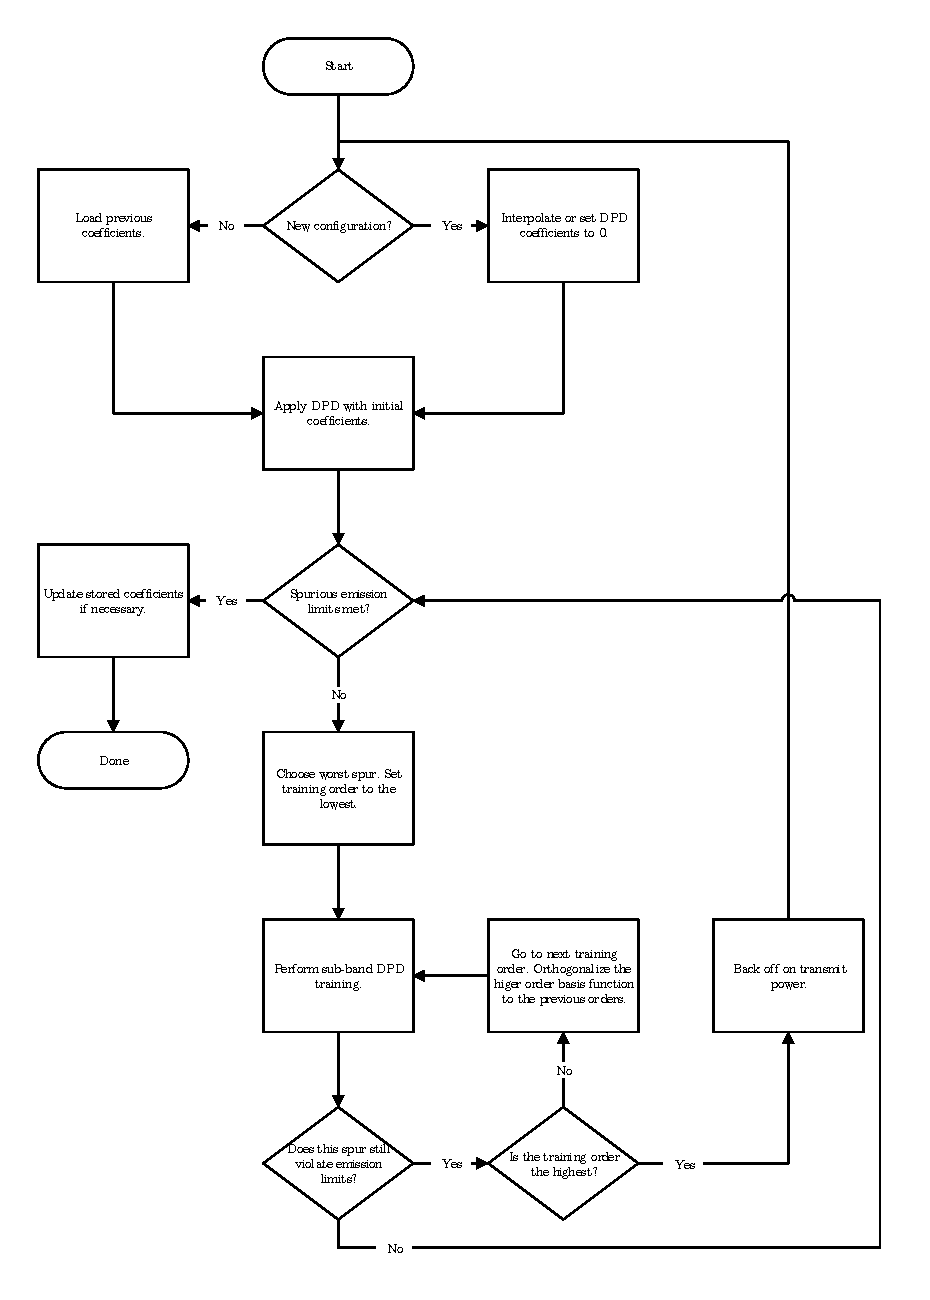
\includegraphics[width=0.89\textwidth]{SubBandSystemNew.pdf}}
	\caption[]{Flow chart of the proposed iterative sub-band DPD solution.}
	\label{fig:SystemFlowChart}
\end{figure*}
In this section, the overall flow of the proposed DPD processing is summarized and presented, thus putting all the bits and pieces together. 
Fig. \ref{fig:SystemFlowChart} presents a flow chart illustrating the overall DPD system processing including the iterative IMD learning and sequential learning for the higher nonlinearity orders.

The system begins by applying stored coefficients if they are available. 
If they are not available, the system will interpolate from other previously stored values if possible or set the DPD coefficients to zero. 
The system searches for spurious emissions in violation of a threshold. 
If there is a violation, the system chooses the most extreme violation to train on. 
We then choose the lowest possible order to train on for that spur (third for IM3, fifth for IM5, etc.) and perform a sub-band DPD learning step after which the spurious emissions are checked to see whether they already meet the emission requirements or not. 
If they do not satisfy emission requirements, an additional nonlinearity order is added. 
In all the learning phases, the DPD learning rate $\mu$ is varied according to the residual correlation between the observed IMD emissions and the corresponding basis function(s), in order to improve the learning speed, as explained in Algorithm \ref{alg:mu}. 

Once the spurious emission is below the threshold, we search for another spur that is above the limit. If there is one, we will similarly train on that spur. We then begin the search again realizing that it is possible that a previously trained spur may no longer meet the requirements due to the mutual effects of one DPD application on the other. In the case that the DPD can not sufficiently suppress the spurious emission below the limit, we lower the transmit power and begin again. Whenever all spurs are under the limit, the coefficients can be stored in the memory.
This serves as a starting point for whenever the transmission scenarios are repeated and for interpolation of other values. 
In the next section, comprehensive experimental results are presented using the \textsc{Warp}Lab setup demonstrating the effectiveness of the proposed DPD solution.

%\import{./}{Section_WarpLabResults.tex}
\section{\textsc{Warp}Lab Results}
\label{sec:WARPLabResults}
The methods presented previously in the paper were tested using the \textsc{Warp}Lab framework on the \textsc{Warp}v3 board. 
\textsc{Warp} is a software-defined radio platform that allows for rapid prototyping by interfacing with \textsc{Matlab} to perform the baseband signal processing  \cite{warpProject}. 
A photo of the experimental setup is shown in Fig. \ref{fig:exp_setup}. 
For these experiments, the DPD processing is done on the host CPU, but the broadcasting is done on the \textsc{Warp} radio hardware which includes the Maxim MAX2829 transceiver and the Anadigics AWL6951 PA.

\begin{figure}[]
	\centering
	%\vspace{0.5cm}
	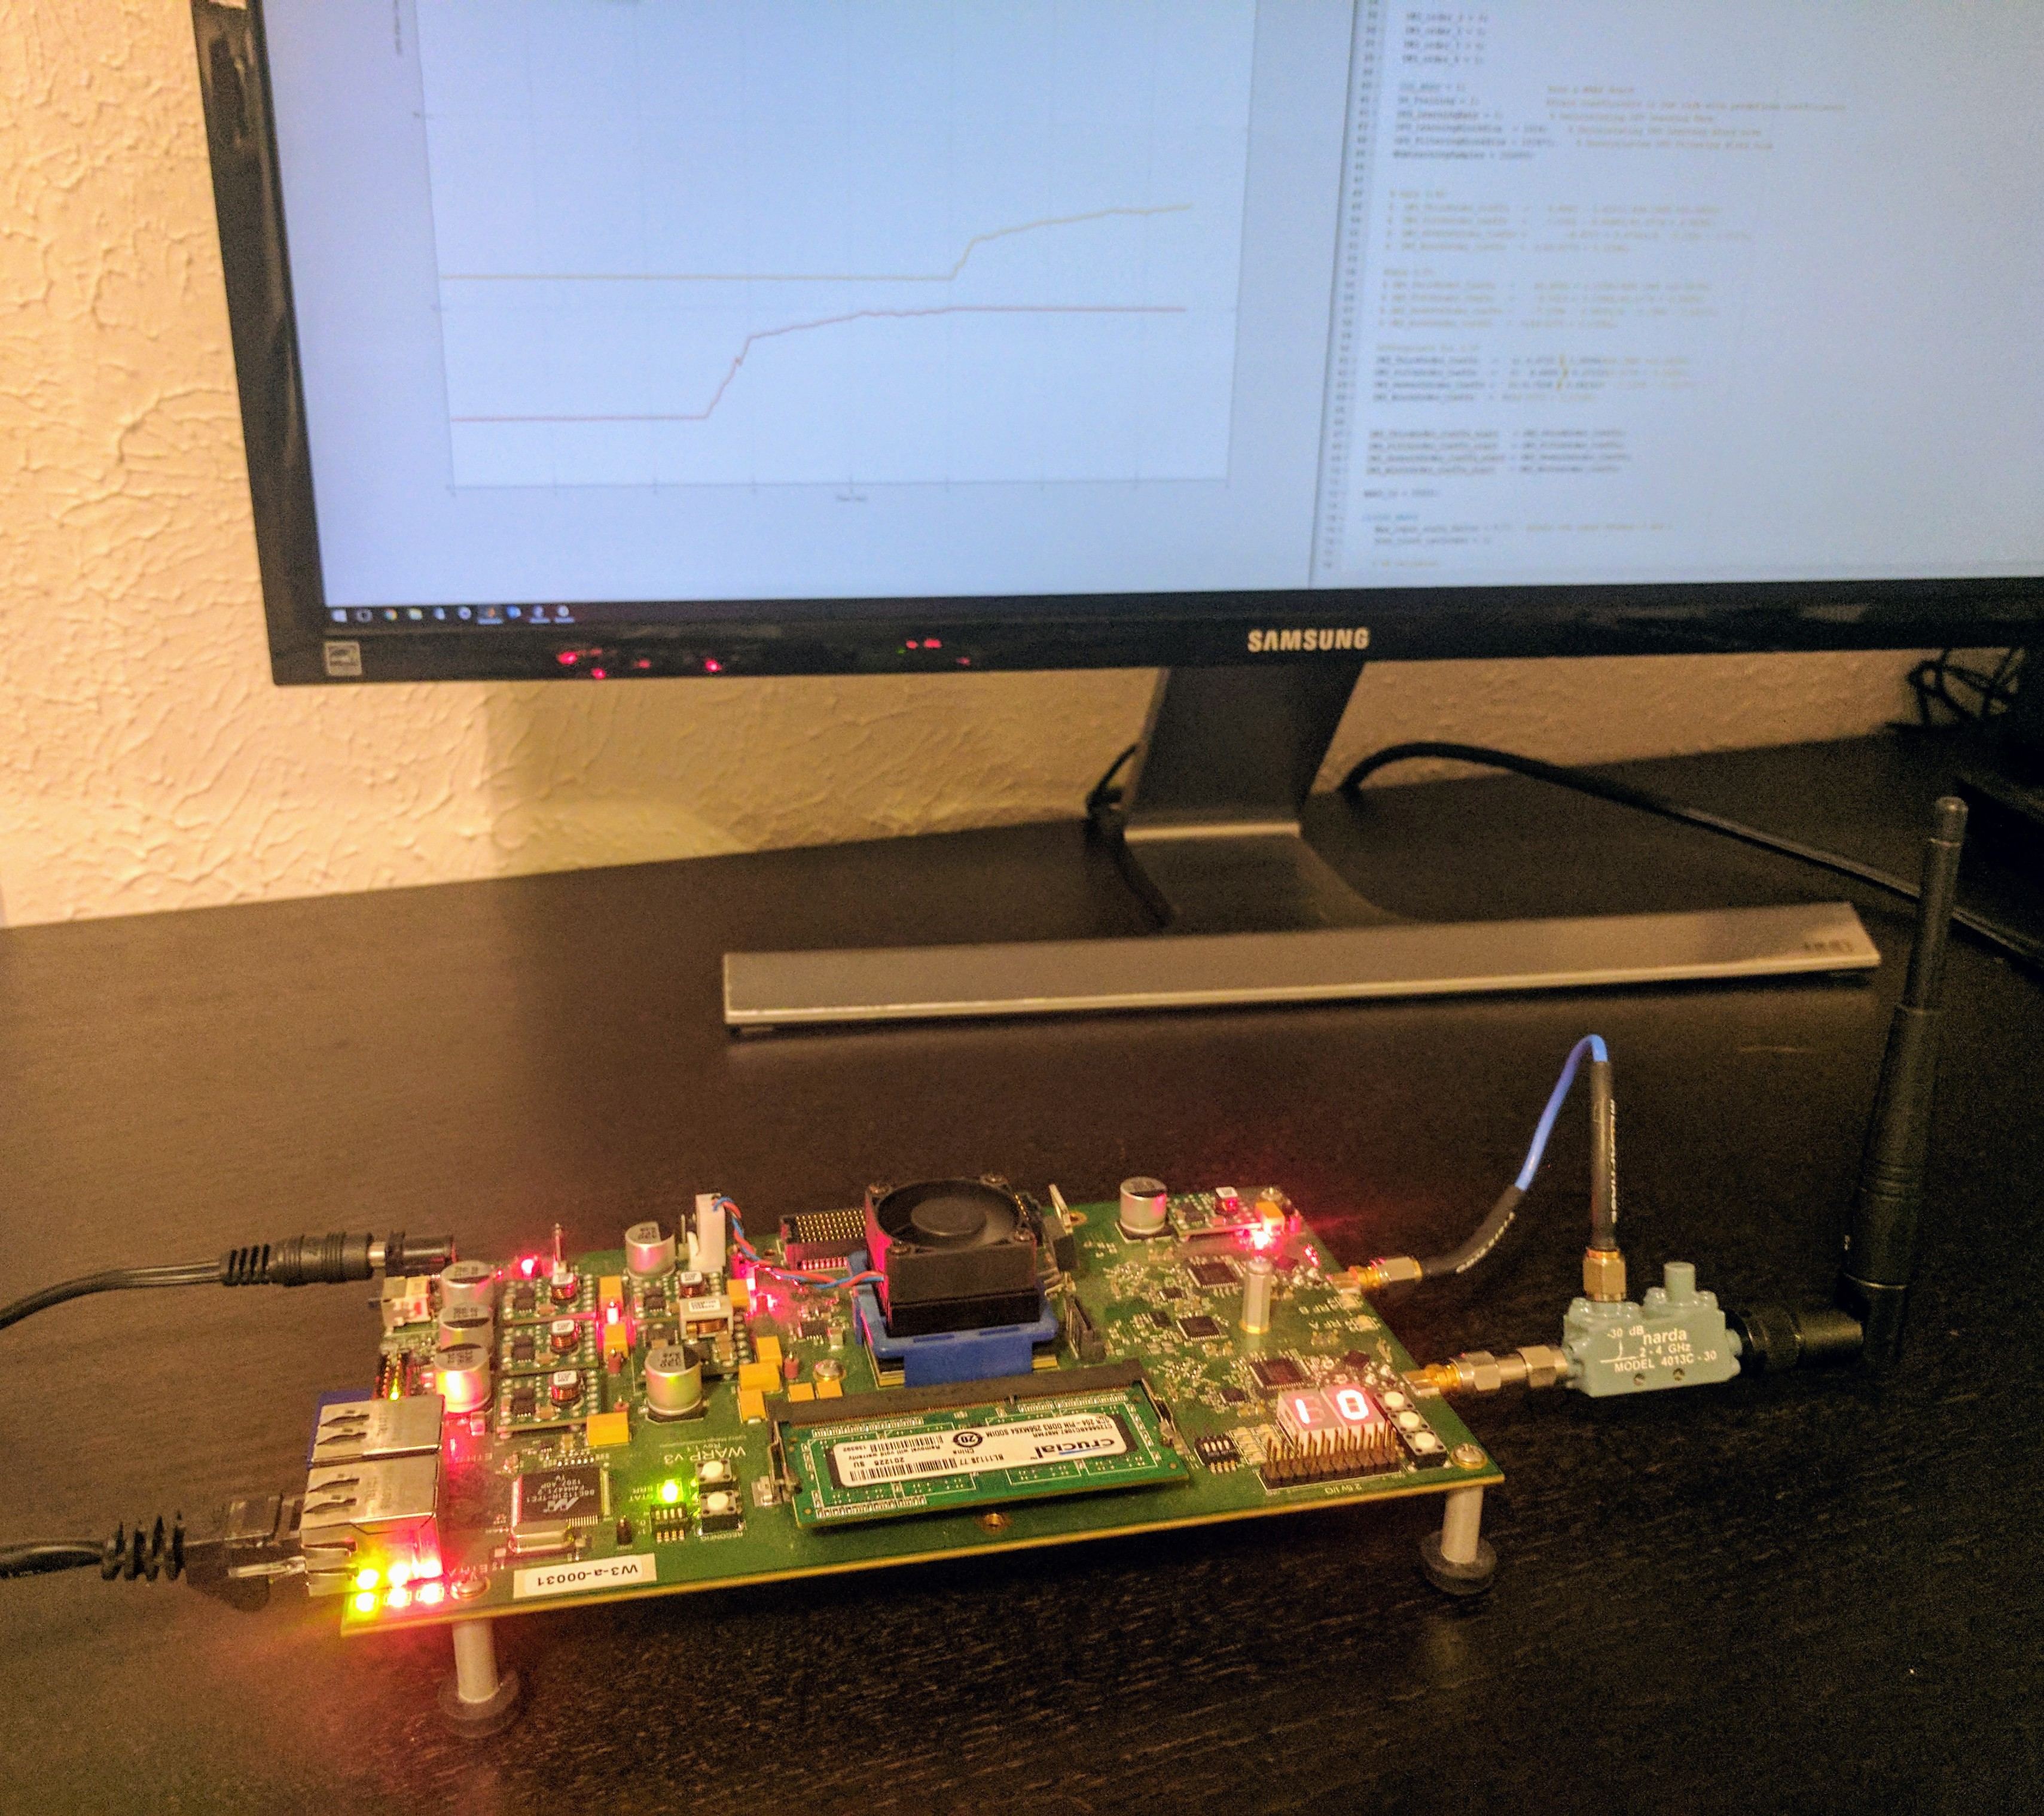
\includegraphics[width=0.75\columnwidth]{Setup.jpg}
	\caption{The \textsc{Warp}v3 board interfaces with \textsc{Matlab} via an Ethernet cable connected to a PC. The TX port is directly connected to the RX port via a 30 dB directional coupler for the feedback loop during training.}
	\label{fig:exp_setup}
\end{figure}

\subsection{IM3$\pm$ Iterations}
We began by testing the iterative method presented in Section \ref{sec:Analysis}. 
An LTE uplink signal was generated in \textsc{Matlab} with two non-contiguous carriers. 
One carrier was 3 MHz and the other was 1.4 MHz. 
Both carriers had 64 QAM subcarrier modulation. 
The frequency domain results at each iteration are shown in Fig. \ref{fig:RightThenLeft}. 
The IM3+ spur was trained first using seventh-order DPD processing, and suppression was achieved as evident in the red curve. 
However, the IM3- spur magnitude was increased slightly which is consistent with (\ref{eq:IM3_-}). 
We then trained the IM3- spur (yellow curve). 
Again, there was a negative effect on the opposite spur, so we retrained the IM3+ spur (purple curve). 
At this point, we were satisfied with the performance and quit training. 

\begin{figure}[t!] 
	\centering
	sing 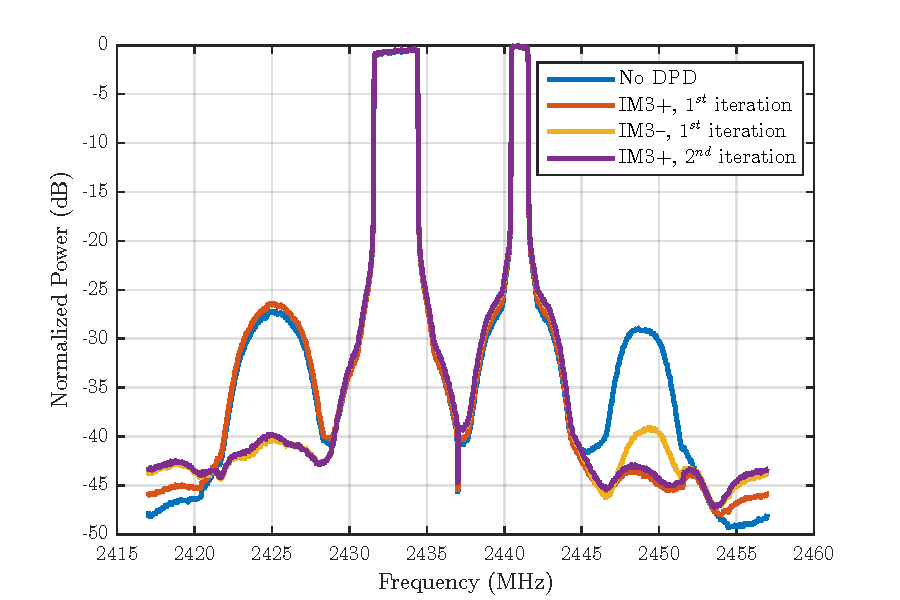
\includegraphics[width=0.9\columnwidth]{RightThenLeft_NEW}
	\caption{Normalized spectral result when using the iterative method to suppress both the IM3+ and the IM3- spurs.}
	\label{fig:RightThenLeft}
\end{figure}

\subsection{Sequential Learning}
As presented in Section \ref{sec:Sequential_Learning}, we then tested the sequential learning concept in \textsc{Warp}Lab where we started with low-order nonlinearities and added higher orders as needed. 
In Fig. \ref{fig:ConcurrentConvergence}, we show an example for comparison using the previously developed concurrent training method. 
We then switched to using the new sequential method as seen in Fig. \ref{fig:SequentialConvergence}. For these two experiments, the same LTE uplink signal and setup were used. 
We see that all the coefficients converged to approximately the same value. 
In Fig. \ref{fig:IterativeSpectrumvsConcurrent}, we show the results in the frequency domain on the IM3+ spur. 
From these figures, it is evident that the final result is equivalent and the only difference is the amount of time it takes to train.

\begin{figure}[t!] 
	\centering
	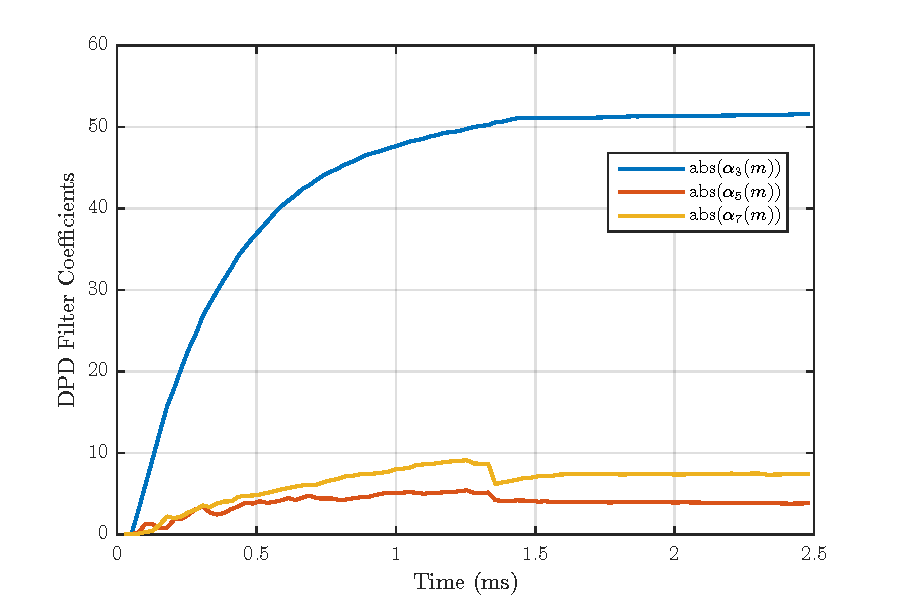
\includegraphics[width=0.9\columnwidth]{ConcurrentConvergence}
	\caption{Example DPD coefficient convergence when concurrent training is used. 
		By training multiple orders concurrently, convergence occurs more rapidly at the price of additional hardware complexity when compared to sequential learning.}
	\label{fig:ConcurrentConvergence}
\end{figure}

\begin{figure}
	\centering
	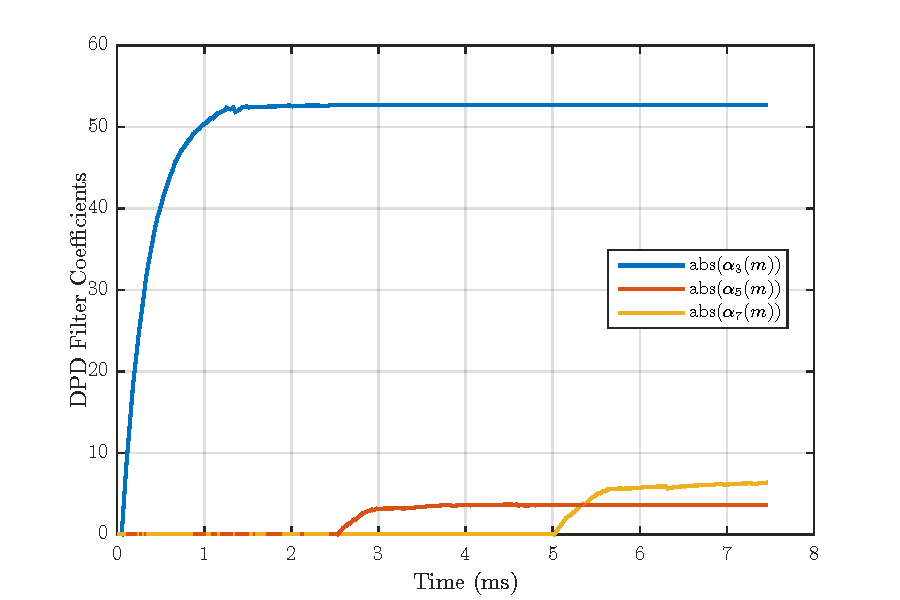
\includegraphics[width=0.9\columnwidth]{SequentialConvergence}
	\caption{\textsc{Warp}Lab testing of sequential learning of DPD coefficients. 
		By training multiple orders sequentially, convergence occurs more slowly with the benefit of less hardware complexity when compared to concurrent learning.}
	\label{fig:SequentialConvergence}
\end{figure}

\begin{figure}[t!] 
	\centering
	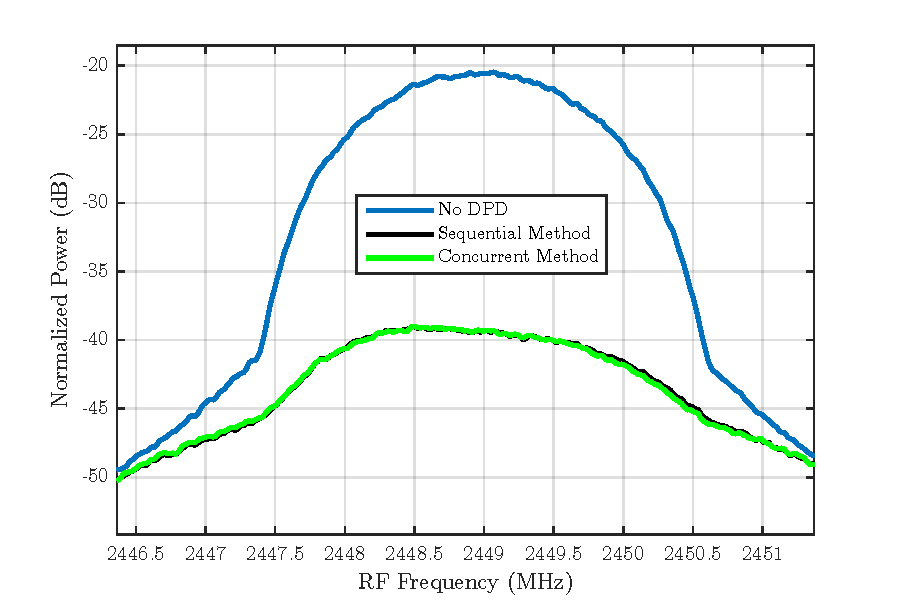
\includegraphics[width=0.9\columnwidth]{IterativeSpectrumvsConcurrent}
	\caption{PSD result when using the concurrent and sequentially trained coefficients to suppress the IM3+ spur. 
		This shows nearly identical performance between the methods.}
	\label{fig:IterativeSpectrumvsConcurrent}
	%\vspace{-10pt}
\end{figure}

\subsection{Speed-up Methods}
The convergence time for sequential training is longer than training in parallel as discussed earlier and shown in Figures \ref{fig:ConcurrentConvergence} and \ref{fig:SequentialConvergence}. 
To overcome this, we tested the previously presented methods for speeding up the convergence time.

\begin{figure}[t] 
	\centering
	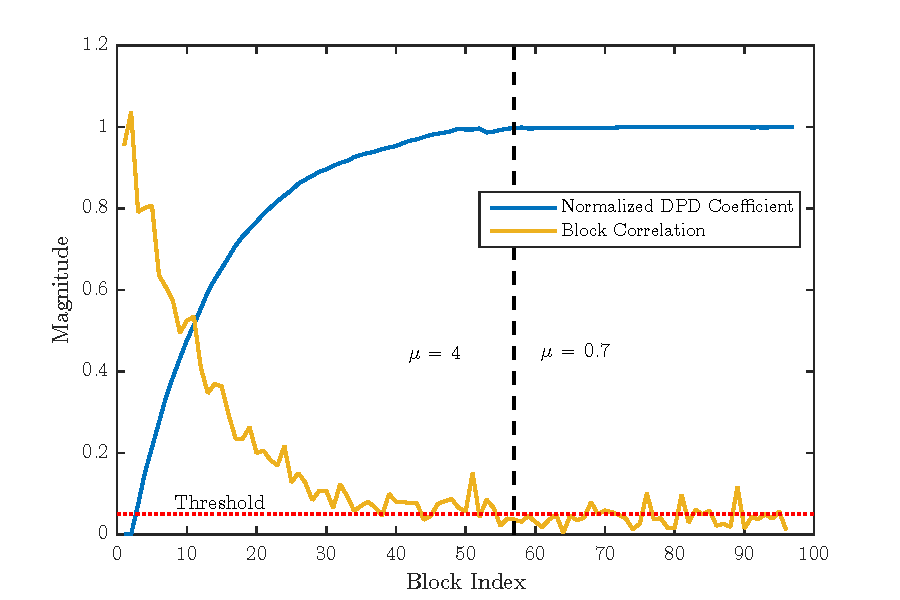
\includegraphics[width=0.9\columnwidth]{Convergence_Mu}
	\caption{Correlation vs. block index during DPD training. 
		As training progresses the correlation decreases. 
		Once it is below the threshold for a total number of times greater than the confidence metric, we change to the lower learning rate.}
	\label{fig:Convergence_Mu}
	%\vspace{-10pt}
\end{figure}

We tested the adaptive $\mu$ concept presented by Algorithm 1. 
In Fig. \ref{fig:Convergence_Mu}, we show the correlation between the error block and the LMS reference block as the algorithm converges. 
As the DPD coefficient convergences (shown in blue), the correlation decreases (shown in orange). 
When it is below the threshold ($\gamma$) of 0.05 (shown in red) more than 5 times (the confidence metric, $\nu$), the learning rate changes from $\mu = 4$ to $\mu = 0.7$. 
This change of $\mu$ is denoted by the dashed line. 
The values were determined experimentally to what worked well for a variety of scenarios as determined by the authors. 

We then tested the concept of starting the DPD coefficient at a value based off the interpolation of other trained values. 
When using \textsc{Warp}Lab, there is an RF gain parameter that sets the gain for the PA. This value is an integer between zero and sixty-three with approximately half a dB of gain per integer increase of this parameter. We started with an RF gain parameter of 45 where we trained from a starting point of zero. Then, we increased the RF gain to 55 where we again trained from 0. At each, the coefficients converged smoothly with sufficient suppression. 

We then choose to work at an RF gain of 50. We linearly interpolated from the two values previously stored. We then started training from this point. The training is shown in Figure \ref{fig:Interpolate}. Based off the sequential, LMS training, a small update to the interpolation guess is made. 

\begin{figure}[t!] 
	\centering
	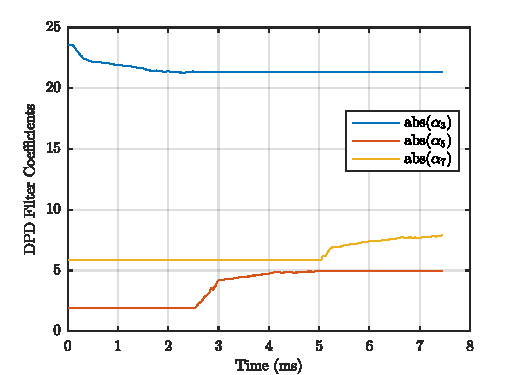
\includegraphics[]{Interpolate} 
	\caption{Convergence of the DPD coefficients after interpolating from previously learned coefficients.}
	\label{fig:Interpolate}
	%\vspace{-10pt}
\end{figure}

As we continue to transmit under various conditions, the interpolations become more accurate. Eventually, a complete table of DPD coefficients is formed. Then whenever we need to broadcast, we can simply load the previous coefficients and quickly update them to account for small fluctuations if needed. 

\subsection{Full System Verification}
We then put everything together in \textsc{Warp}Lab to follow the process shown in Figure \ref{fig:SystemFlowChart} where multiple spurs need to be under a threshold. The previously discussed speed-up methods are applied in the training process. Two LTE carriers are broadcast. The two carriers are set to be 1.4 MHz LTE uplink signals spaced 6 MHz apart. This allowed the IM5 spurs to be observable in the \textsc{Warp} board's 40 MHz RF Bandwidth. For this experiment, we set a threshold that the spurs must be 35 dB below the main carriers. The results are plotted in the Figure \ref{fig:IM5}.

\begin{figure}
	\centering
	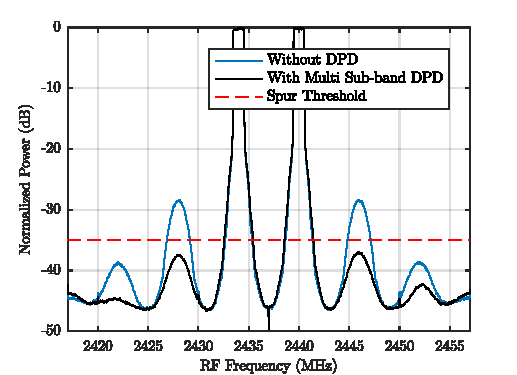
\includegraphics[]{IM5Spectrum}
	\caption{Normalized spectral result when using the iterative method to make sure both IM3 and both IM5 spurious emissions are below the threshold}
	\label{fig:IM5}
\end{figure}

\begin{table}
	\begin{tabular}{c l c|r r r r}
		
		\multicolumn{3}{c|}{Training Step}  & \multicolumn{4}{c}{Result (dB)} \\ 
		\hline 
		Step & Spur & Order & IM5-  & IM3- & IM3+ & IM5+ \\ 
		\hline 
		0 & - & - & -38.7 & -28.0 & -27.9 & -38.8 \\ 
		
		1 & IM3+ & 3 & -37.3 & -27.4 & -34.4 & -36.7 \\ 
		
		2 & IM3+ & 5 & -37.2 & -27.4 & -36.9 & -36.4 \\ 
		
		3 & IM3- & 3 & -35.9 & -33.9 & -35.5 & -34.9 \\ 
		
		4 & IM3- & 5 & -35.0 & -37.0 & -35.8 & -34.5 \\ 
		
		5 & IM5+ & 5 & -34.5 & -33.15 & -34.5 & -43.0 \\ 
		
		6 & IM3- & 5 & -33.6 & -37.1 & -34.3 & -44.4 \\ 
		
		7 & IM5- & 5 & -42.9 & -32.0 & -33.5 & -44.0 \\ 
		
		8 & IM3- & 5 & -45.1 & -37.6 & -33.2 & -44.0 \\ 
		
		9 & IM3+ & 3 & -43.2 & -32.3 & -36.8 & -42.6 \\ 
		
		10 & IM3- & 5 & -44.6 & -37.5 & -37.0 & -42.5 \\ 
		
	\end{tabular} 
	\caption{Results of the intermediate training steps in the multi sub-band DPD from Figure \ref{fig:IM5}.}
	\label{tab:IM5}
\end{table}

We assume this to be a new configuration where we start with no know coefficients; every coefficient gets initialized to zero. The non-contiguous signal is broadcast over the \textsc{Warp} board, and the spectrum for this is shown as the blue curve in Figure \ref{fig:IM5}. We identify the IM3+ spur as the most severe and train on it. There is some suppression, but it does not completely meet the threshold. We train another order on the IM3+ spur and then continue the process until the final result shown in black is achieved. During the process, the mutual effect of one DPD training negatively impacts the other spurs and causes additional steps in the multi sub-band DPD. All of the intermediate results are shown Table \ref{tab:IM5}.



%\begin{figure}[t!] 
%\centering
%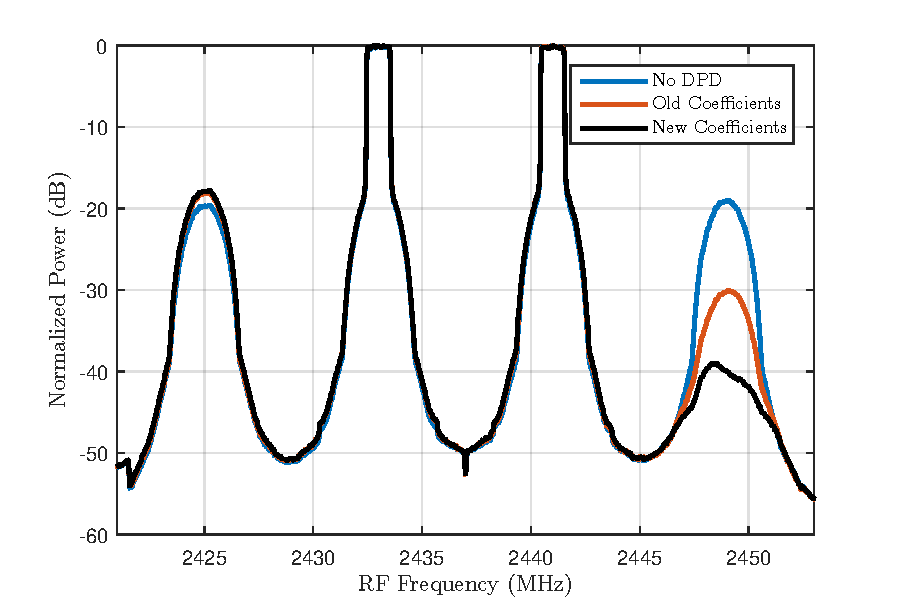
\includegraphics[width=\columnwidth]{Figures/UseOldCoeff_IncreasePower_PSD}
%\caption{}
%\label{fig:UseOldCoeff_IncreasePower_PSD}
%\end{figure}





\section{Conclusion}
In this paper an iterative, multi sub-band DPD learning algorithm has been presented that can suppress the IM3 and IM5 spurious emissions. 
A sequential learning procedure where higher nonlinearity orders were added one at a time was also presented in order to reduce the complexity and add flexibility to the DPD solution. 
Additionally, the convergence speed of the proposed DPD has been improved by two methods, while not sacrificing the DPD performance. 
The first used a variable learning rate which switches from high speed to lower speed once the loop becomes close to convergence. 
The second method starts the DPD learning from previously learned points and uses interpolation of past scenarios to reduce convergence time. 
A \textsc{Warp}Lab implementation of the proposed DPD solution has been demonstrated showing excellent performance with up to 20 dB suppression in the undesired spurious emissions.

%\begin{acknowledgements}
%If you'd like to thank anyone, place your comments here
%and remove the percent signs.
%\end{acknowledgements}

% BibTeX users please use one of
%\bibliographystyle{spbasic}      % basic style, author-year citations
%\bibliographystyle{spmpsci}      % mathematics and physical sciences
%\bibliographystyle{spphys}       % APS-like style for physics
\bibliographystyle{ieeetr} 
\bibliography{Ref}   % name your BibTeX data base

\iffalse %Comment out the template bib and other things I might want to look at

\begin{figure}
% Use the relevant command to insert your figure file.
% For example, with the graphicx package use

\includegraphics{example.eps}
% figure caption is below the figure
\caption{Please write your figure caption here}
\label{fig:1}       % Give a unique label
\end{figure}
%
% For two-column wide figures use
\begin{figure*}
% Use the relevant command to insert your figure file.
% For example, with the graphicx package use

\includegraphics[width=0.75\textwidth]{example.eps}
% figure caption is below the figure
\caption{Please write your figure caption here}
\label{fig:2}       % Give a unique label
\end{figure*}
%
% For tables use
\begin{table}
% table caption is above the table
\caption{Please write your table caption here}
\label{tab:1}       % Give a unique label
% For LaTeX tables use
\begin{tabular}{lll}
\hline\noalign{\smallskip}
first & second & third  \\
\noalign{\smallskip}\hline\noalign{\smallskip}
number & number & number \\
number & number & number \\
\noalign{\smallskip}\hline
\end{tabular}
\end{table}

% Non-BibTeX users please use
\begin{thebibliography}{}
%
% and use \bibitem to create references. Consult the Instructions
% for authors for reference list style.
%
\bibitem{RefJ}
% Format for Journal Reference
Author, Article title, Journal, Volume, page numbers (year)
% Format for books
\bibitem{RefB}
Author, Book title, page numbers. Publisher, place (year)
% etc
\end{thebibliography}
\fi

\end{document}
% end of file template.tex

